% A Tale of Two Slinkies: Learning about Model Building in a Student Driven Classroom
%
% Calvin Berggren, Punit Gandhi, Jesse Livezey, Ryan Olf
%
% 2013-08-??: v1
%
\documentclass[prb,preprint,superscriptaddress]{revtex4-1} 

\usepackage{graphicx}
\usepackage{hyperref}
\usepackage{amsmath}
\usepackage{amsfonts} % needed for bold Greek, Fraktur, and blackboard bold
\usepackage{amssymb}
\usepackage[margin=1in]{geometry}
\usepackage{dcolumn}
\usepackage{multirow}
\usepackage{tikz}
\usetikzlibrary{calc,patterns,decorations.pathmorphing,decorations.markings}

% TODO: remove these lines, which expand the margins (useful for comments)
\textwidth  .72\paperwidth
\hoffset -1in
\oddsidemargin .14\paperwidth
\evensidemargin .14\paperwidth
\marginparwidth .11\paperwidth


% Draft macros
\usepackage[normalem]{ulem} % for strikethrough
\usepackage[usenames,dvipsnames]{xcolor}
\newcommand{\TODO}[1]{\marginpar{\raggedright\scriptsize\textbf{TODO:} #1} (\textbf{TODO})}
\newcommand{\NOTEMARG}[1]{\marginpar{\raggedright\scriptsize\textbf{NOTE:} #1} (\textbf{NOTE})}
\newcommand{\NOTE}[1]{\marginpar{\footnotesize\textbf{NOTE}} (\textbf{NOTE: #1})}
\definecolor{purple}{rgb}{1,0,1}
\newcommand{\calvin}[2]{\textcolor{purple}{\sout{#1}#2}}

\newcommand{\eq}[1]{eq.~\eqref{eq:#1}}
\newcommand{\eqs}[2]{eqs.~\eqref{eq:#1} and \eqref{eq:#2}}
\renewcommand{\sec}[1]{section~\ref{sec:#1}}
\newcommand{\secs}[2]{sections~\ref{sec:#1} and \ref{sec:#2}}
\newcommand{\subsec}[1]{section~\ref{subsec:#1}}
\newcommand{\subsubsec}[1]{section~\ref{subsubsec:#1}}
\newcommand{\app}[1]{appendix~\ref{app:#1}}
\newcommand{\fig}[1]{figure~\ref{fig:#1}}
\newcommand{\figs}[2]{figures~\ref{fig:#1} and \ref{fig:#2}}
\newcommand{\tab}[1]{table~\ref{tab:#1}}
\newcommand{\nn}{\nonumber}

\newcommand{\FIGstudents}{
\begin{figure}[t]\center
\includegraphics[width=\columnwidth]{FIGstudents.pdf}
\caption{\label{fig:students} Students from the 2012 Compass Project summer program with model slinkies built out of washers and rubberbands.}
\end{figure}
}


\newcommand{\FIGpulsedrop}{
\begin{figure}[t]\center
\includegraphics[width=\columnwidth]{FIGpulsedrop.pdf}
\caption{\label{fig:pulsedrop} A few frames from a slow motion image of a wave pulse sent down a slinky next to a falling slinky.  Possible a graph of position vs time of the top of the falling slinky and the wave pulse.}
\end{figure}
}


\begin{document}

\title{A Tale of Two Slinkies: Learning about Model Building in a Student Driven Classroom}
\author{Calvin Berggren}
\email{calvin1414@berkeley.edu}
\affiliation{Department of Physics, University of California at Berkeley, Berkeley, CA 94720, USA}
\affiliation{Berkeley Center for Theoretical Physics, University of California at Berkeley, Berkeley, CA 94720, USA}
\affiliation{Theoretical Physics Group, Lawrence Berkeley National Laboratory, Berkeley, CA 94720, USA}
\author{Punit  Gandhi}
\email{punit\_gandhi@berkeley.edu}
\author{Jesse Livezey}
\email{jesse.livezey@berkeley.edu}
\author{Ryan Olf}
\email{ryanolf@berkeley.edu}
\affiliation{Department of Physics, University of California at Berkeley, Berkeley, CA 94720, USA}
\date{\today}

\begin{abstract}

We describe a set of conceptual activities and hands-on experiments based around understanding the dynamics of a slinky that is hung vertically and released from rest.
The motion, or lack thereof, of the bottom of the slinky after the top is dropped challenges students' expectations and provides motivation and context for learning about scientific model building.
%This curriculum was developed for a week-long summer program for incoming freshmen as a part of the Compass Project~\cite{albana2013},
%The summer program is the first part of a three-course sequence aimed at helping incoming students in the physical sciences develop their identity as scientists.
This curriculum helps students learn about the model building process by giving them an opportunity to enlist their collective intellectual and creative resources to develop and explore two different physical models of the falling slinky system. By engaging with two different models, students not only have the opportunity to understand an intriguing counterintuitive phenomenon from multiple perspectives, but also learn deeper lessons about the nature of scientific understanding, the role of physical models, and the experience of doing science. 
The sequence of activities we present were developed for a week-long summer program for incoming freshmen as a part of the Compass Project,~\cite{albana2013} but could easily be implemented in a wide range of classrooms at the high school and introductory college levels.
\end{abstract}

\maketitle

\section{Introduction}
The basis for the curriculum presented in this work is an experiment involving a
slinky that is hung vertically and released from rest, colloquially known as a ``slinky drop."
 \NOTEMARG{Add multi-frame figure with labels. (Jesse)}
The experiment typically lasts a fraction of a second, but when observed in slow motion one sees the slinky compress from the top down while the bottom portion remains at rest---naively seeming to defy gravity---until the slinky has completed its collapse. 
\footnote{One can demonstrate experimentally that the center of mass of the slinky falls in accordance with Newton's Laws, although here we confine ourselves to addressing the lack of motion of the bottommost potion of the slinky.}
The slinky drop experiment and other related phenomena have
been studied in detail\cite{calkin1993, newburgh1995, graham2001, aguirregabiria2007,unruh2011, cross2012}
and have recently attracted a flurry of interest online \cite{..}.
In this work, we describe how we used the slinky drop phenomenon to teach the modeling process by giving
 the students first-hand experience constructing two distinct but complementary physical models.

This curriculum was developed for an intensive one-week summer course for
incoming freshmen as a part of the Compass Project~\cite{albana2013,Roth2012,drdf2013a,drdf2013b} and was
presented in a student-driven classroom inspired by Modeling Instruction\cite{hestenes1987}.
Students in the class shared a common interest in the physical sciences but came from diverse backgrounds with widely varying levels of preparation. In spite of this, it was important that all students be able to contribute to and take ownership of the models developed in the course. The slinky drop phenomenon strikes a delicate balance between competing pedagogical needs. The setup is simple enough that even less prepared students have (incorrect) intuition for what should happen, and can therefore be surprised by the observed (contradictory) result, which engages the students interest and motivates further exploration. On the other hand, a satisfactory intuitive %(let alone quantitative) 
understanding of the phenomenon is both a) attainable to a wide range of students and b) sufficiently challenging that such students can begin their exploration on a relatively level playing field, facilitating collaboration and shared learning.

During the course of the program, students approached the slinky drop problem using two complementary models.
In one approach, detailed in \sec{forces}, students approximate
the slinky as a number of discrete masses connected by simple springs and applied
 Newton's Laws to calculate the motion of these masses.
In the second, complementary
approach, students model the propagation of information, as detailed in \sec{information}. This model
describes the event when the slinky is released as a piece of information that
needs to travel to other parts of the system---via either a wave pulse or the shock wave of medium collapse---before they are able to respond.
Information initially proved to be a more challenging concept for the
students to grasp but ultimately provided a clearer, more intuitive way of understanding why the bottom
remains stationary. After presenting each
model individually in \secs{forces}{information}, we compare the models and
discuss model building in general in \sec{discussion}.
% Finally, our conclusions are presented in \sec{conclusion}.

\section{Modeling the slinky using discrete masses}
\label{sec:forces}

\begin{figure*}[t]
\centering

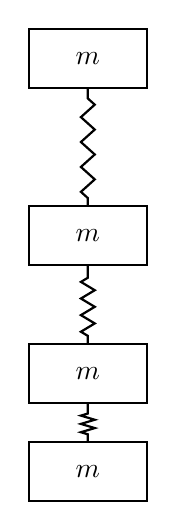
\begin{tikzpicture}[every node/.style={draw,outer sep=0pt,thick}]
\tikzstyle{mass}=[minimum width=1.5cm,minimum height=0.75cm,anchor=north]
\tikzstyle{spring}=[thick,decorate,decoration={zigzag,pre length=0.1cm,post length=0.1cm}]

\node (M1) [mass] {$m$};

\node (M2) at (M1.south) [mass,yshift=-1.5cm] {$m$};
\draw [spring,decoration={segment length=9}]
   (M2.north) -- ($(M1.south east)!(M2.north)!(M1.south west)$);

\node (M3) at (M2.south) [mass,yshift=-1cm] {$m$};
\draw [spring,decoration={segment length=6}]
   (M3.north) -- ($(M2.south east)!(M3.north)!(M2.south west)$);

\node (M4) at (M3.south) [mass,yshift=-0.5cm] {$m$};
\draw [spring,decoration={segment length=3}]
   (M4.north) -- ($(M3.south east)!(M4.north)!(M3.south west)$);

\end{tikzpicture}

\caption{A model of the slinky using discrete masses connected by springs.}
\label{fig:discrete}
\end{figure*}

In this model (the ``discrete model''), students use forces and Newton's Laws to calculate the
motion of the slinky in free fall. This
model is conceptually straightforward and allows students to follow a
reductionist approach wherein they divide the slinky into intuitively and mathematically accessible
constituents. In particular, students break the model slinky into a series of discrete masses connected by simple springs,
as shown in \fig{discrete}.
Students can then apply familiar concepts in deciding how to model each part. The equations of motion that result from this simple model are quite difficult to solve analytically for slinkys composed of more than a few masses, but the model is still very useful in understanding the slinky drop in particular, and model building in general. 

In developing this model, students face many choices regarding approximations and simplifications. Which choices that render the mathematics more tractable, such as choosing to model only a few masses, yield a system that reproduces ``levitation'' phenomenon? What roles do the various parameters of the model---number, mass, spring constant---play in reproducing the relevant qualities of a slinky? To answer these questions, and to glean insight into the slinky drop, the students explore the model in two complementary ways: In section \ref{subsec:forcesexperiment} they build and study a physical approximation of the discrete system, while in section \ref{subsec:forcesnumeric} they numerically evolve the derived equations of motion.


% The strategy  was to find the forces (gravity and elastic) acting on 
% each mass as a function of position and then
% apply Newton's Laws to find the resulting motion.

%% no need for outline
% We then attempted to solve the equations
% of motion numerically to find the motion (\subsec{forcesnumeric}).

\subsection{Physical realization of the discrete model}
\label{subsec:forcesexperiment}

In order to be useful for understanding the the slinky drop, the discrete model needs to be able to reproduce the essential physics of the slinky. To learn about the applicability and limitations of the discrete model, and the implications of the various choices involved in defining it, the students built physical realizations of the model using masses (washers, nuts) tied to springs (rubber bands, stretchy silicone).  The motion of physical models built using different parameters were compared and contrasted with each other and the motion of the actual slinky.  Example physical models are show in examples are shown in \ref{fig:students}.  

The primary focus of student investigation is whether, and under what circumstances, the physical mass and spring models demonstrate the levitation effect that they seek to understand.  To do this, students build many models with different masses and springs and note the manner in which they drop, as recorded by a high speed camera. From these observations, the students learn which physical properties of the slinky allow for the bottom to remain stationary when the top was released.  In particular, the students realize that the models must be very "stretchy" in order to for this phenomenon to be pronounced.  Further, the students begin to appreciate how extremely stretchy the slinky is relative to other objects.

\begin{figure*}[t!]
  \centering

  \begin{tabular}{cccc}
    \multicolumn{2}{c}{
      \multirow{2}{*}{
        \raisebox{0\height}[0.6\height]{
          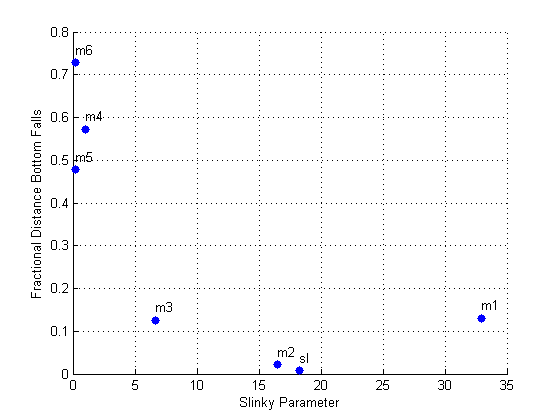
\includegraphics[width=0.5\textwidth]{figs/SlinkyParameter}
        }
      }
    } &
    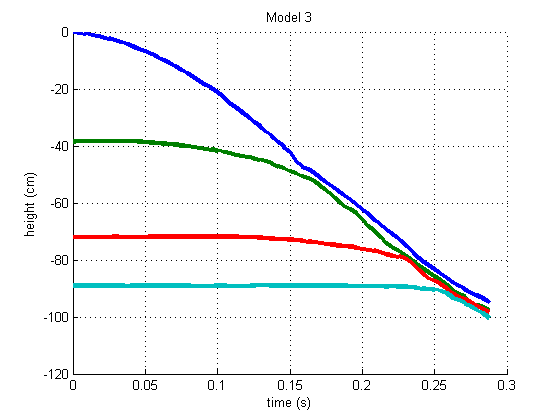
\includegraphics[width=0.25\textwidth]{figs/Slinky3} &
    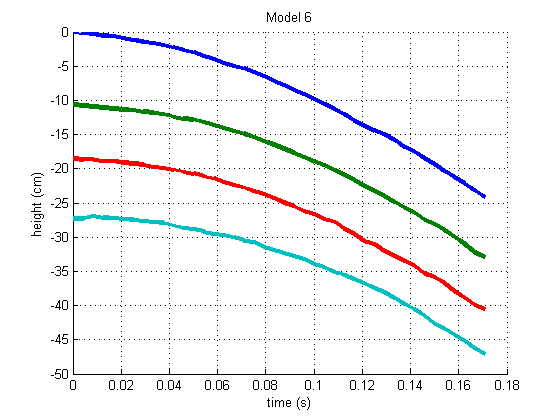
\includegraphics[width=0.25\textwidth]{figs/Slinky6} \\
    \multicolumn{2}{c}{} &
    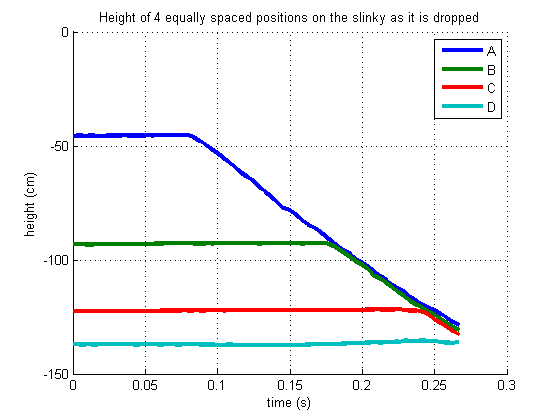
\includegraphics[width=0.25\textwidth]{figs/SlinkyTabs} &
    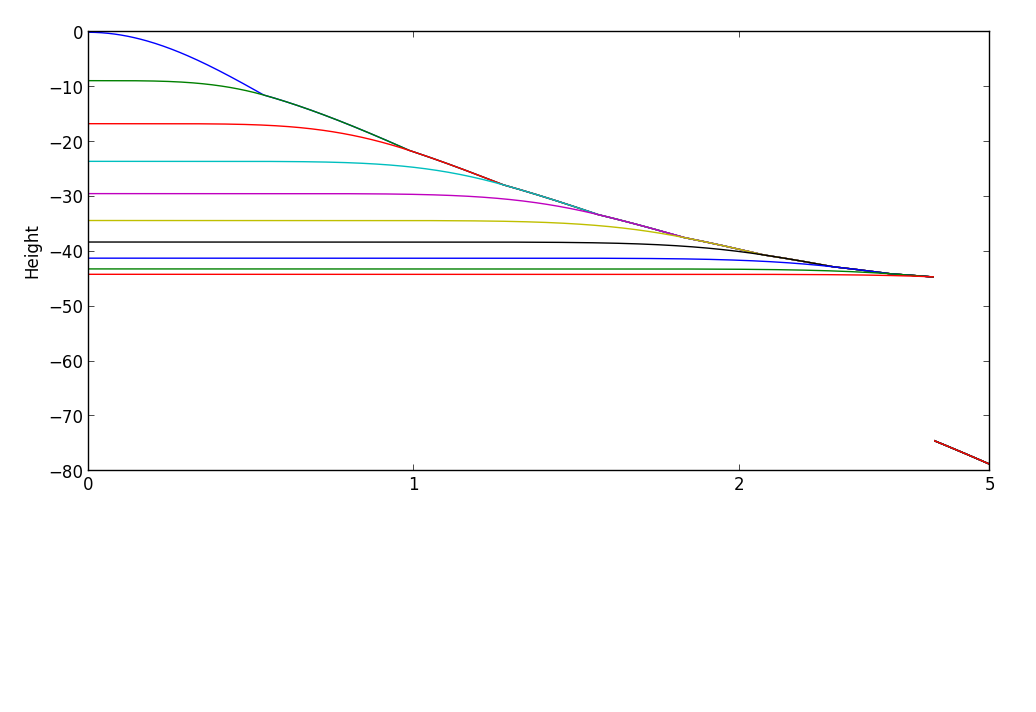
\includegraphics[width=0.25\textwidth]{figs/SlinkySim} \\

  \end{tabular}

  \caption{The left panel shows the correlation of the slinkiness parameter with
           how stationary the bottom mass is. Specifically, the extent to which the
           bottom mass is stationary is measured as the distance the bottom mass falls
           reletive to the stretched length of the system, during the time in which
           the top mass falls the full stretched length. The set of figures in the
           right panel shows the position as a function of time of four positions
           on the system. The top left is Model 3, the top right is 4 masses connected
           by strings, the bottom left is the slinky, and the bottom right is a
           simulation of Model ?.}
  \label{fig:discretemodel}
\end{figure*}

\TODO{Motivate this defninition.}This stretchiness can be characterized by how much the object stretches
under it's own weight as it is suspended.   We can define a slinky parameter as a measure of this:

\begin{equation}
\mathcal{S}=\frac{L_h-L_0}{L_0}
%\mathcal{S}=\frac{m g}{k_\text{eff} L_0 },
\end{equation}
where $L_h$ is the stretched length when suspended vertically and allowed to come to rest, and $L_0$ is the unstretched equilibrium length
when no forces act on it.  It can be shown using Newton's Laws that in the case of the discrete masses and springs model,
this stretching is actually proportional to the total mass $m$ and inversely proportional to the total effective spring constant $k_{\text{eff}}$ of the object.
This is also true in the case of a continous model of the slinky that can support the transmission of waves.  The following dimensionless quantity
can be constructed from the parameters of interest in the problem,
\begin{equation}
\mathcal{S'}=\frac{m g}{k_\text{eff} L_0 },
\end{equation}
 and is infact proportional to the  slinky parameter defined above.  Here, $m$ is the total mass of the object, $g$ is the gravitational acceleration felt as it is suspended, $k_\text{eff}$ is the effective spring constant of the entire object, and $L_0$ is the unstretched length.  It can be a useful activity to experimentally 
confirm this proportionality, particularly when the target audience hasn't been previously exposed to Newton's laws.

Now, in order to see that this parameter is a useful determining the "slinkiness", we must first choose a measure that allows us to compare how closely a model
with a given set of parameters behaves like a slinky in the drop experiment.  Since the phenomena of interest is the lack of motion of the bottom of the slinky, 
a good candidate could be the distance the bottom of the model falls in the time it takes for the model to collapse.  Figure \ref{} shows a plot of this distance, normalized by the stretched length unstretched length amount the object has stretched, for models over a range of different slinky parameters.  The slinky and simulations are also included in this graph.  One can see that the greater the slinky parameter, the less the bottom moves.  (or is there a threshold slinky parameter where  the bottom doesn't move beyond?).  We considered models with 4 masses, and have also shown the positions of the four masses as a function of time.  In order to facilitate comparisons between the models, the positioins have been normalized by the stretched length $L_h$, and the time is measured in units of $\sqrt{m/k_{\text{eff}}}$ of each of model.  

%  \begin{table}[ht]
%  \caption{Model Slinkies} % title of Table
%  \centering % used for centering table
%  \begin{tabular}{c c c c c c} % centered columns (4 columns)
%  \hline\hline %inserts double horizontal lines
%   & m (g) & $k_\text{eff}$ (N/m) & $L_0$ (cm) & $L_h/L_0$ & $\mathcal{S}$ \\ [0.5ex] % inserts table 
% % heading
% \hline % inserts single horizontal line
% model 1 & 405 & 0.7 	& 17   & 5.6	& 34		\\ % inserting body of the table
% model 2 & 205 & 0.7	& 17   & 9.5	& 17		\\
% model 3 & 200 & 2.1	& 14   & 6.5	& 7		\\
% model 4 & 30   & 2.1	& 14   & 2.0	& 1		\\
% model 5 & 200 & 60	& 16   & 2.1	& 0.2		\\
% model 6 & 200 & 75	& 16   & 1.7	& 0.17		\\
% slinky     & 190 & 1.7   & 5.7   & 24	& 19.6		\\ [1ex] % [1ex] adds vertical space
% \hline %inserts single line
% \end{tabular}
% \label{table:slinkies} % is used to refer this table in the text
% \end{table}

\subsection{Numerically testing the discrete model}
\label{subsec:forcesnumeric}

Having taken the step toward understanding the slinky using a model with
discrete masses separated by springs, we sought to make further progress by
solving this model numerically. The students spent some time constructing the
force equations for an $N=4$ system, for example,
%%%
\begin{align} \label{eq:coupleddes}
ma_i &= mg + k(x_{i+1} - x_i) - k(x_i - x_{i-1})
\,,\end{align}
%%%
where $m$ is the mass of each discrete mass, $k$ is the spring constant of each
spring, and $x_i$ and $a_i$ refer to the absolute position and acceleration of each mass.

Doing any serious exploration of these coupled differential equations
analytically was beyond the level of our audience; however, we briefly allowed
the students to consider how they would solve the system in order to demonstrate
the great difficulty of this strategy.

Students were gradually led toward an alternative numerical approach to solving
the problem that divided the evolution of the system into small time
steps. This was motivated by considering examples like the frames in a
movie, such as the slow-motion movies we used to view the slinky. Discretizing time expanded on our previous decision to discretize the mass
in the slinky.

The students were asked to construct an algorithm
for how to proceed from one time step to the next. With the acceleration at each
step given by the force as in \eq{coupleddes}, the students settled on the
following simple algorithm (also known as the Euler method (Ref. \ref{..})),
\TODO{find textbook reference for Euler method}
%%%
\begin{align} \label{eq:algorithm}
v_i(t+\Delta t) &= v_i(t) + a_i(t)\Delta t
\,,\nn\\
x_i(t+\Delta t) &= x_i(t) + v_i(t)\Delta t
\,,\end{align}
with the time step given by $\Delta t$.

With the algorithm in hand, we had the students ``simulate'' the masses and
springs model as a group. Each mass was represented by a group of 
students, who completed the calculations for their mass to figure out where it would be
at the next time step.
% Students were divided into different roles, with some responsible 
% for calculation, others for communicating their position to other groups who 
% needed the information for their own calculations, and others for plotting the results on a graph 
% at the front of the room.
They would also plot their position on the main chalkboard allowing the whole class to track
the progress of the simulation.
Groups needed information from other groups in order to complete their calculations,
and the communication of information between groups was intended 
to foreshadow the inherent time delay in the passing of information, explored later in
the week and described in \sec{information}.

The participatory simulation described here provides good practice in building
a model by iteration and highlights the ability of the numerical approach to incorporate changes to the model. After beginning the activity, questions quickly arise, such
as what to do when a mass passes through another mass. Nothing in the set of equations from \eq{coupleddes} prevents
the masses from passing. The students may wish to allow this to happen as an approximation
or they may wish to modify their procedure, perhaps by somehow merging any two masses which have overlaped
in the most recent time step. Follow up questions for discussion or investigation include
the dependence of the simulation on the size of the time step and the number of masses.
In building a simplified model, it also becomes easy to investigate
other situations by adjusting parameters.

A major goal of this part of the curriculum was to show the benefits of building
numerical models. Not only does a numerical model
practically provide a way to make progress over an exact model which may be difficult
to work with, but these models also often provide a greater degree of transparency and
concreteness into how the system is evolving. We provided the class with the
ponderous analytical solutions to the 4-body system after the activity and asked
them how well they could see what was going on compared to the numerical
approach. We also asked how well they expected each approach to be able to
handle kinks or bends in the slinky to demonstrate the benefit numerical
approaches have in handling perturbations.

One potential obstacle with the numerical simulation is that, for an $N$-body simulation and for the algorithm described in \eq{algorithm},
it will take $2N$ time steps for the bottom mass to move. This is not an explanation for
the lack of motion in the real slinky but is rather an artifact of the discretization of time:
the last mass will always wait $2N$ time steps regardless of the size of the step.
This provides an opportunity to discuss one limitation of this model.
% One way to
% accelerate the activity would be to use a more accurate symplectic algorithm, such as the
% symplectic Euler algorithm (Ref. \ref{...}). This algorithm would require only $N$ steps to move the bottom
% mass, partially alleviating the tedium for the last group.

It is also possible to perform this activity using a spreadsheet, which allows the steps to be
calculated much faster, albeit less collaboratively. We had the students implement the algorithm on a spreadsheet once they
felt comfortable with the details of the process. This allowed them to explore some of the follow
up questions more efficiently.

\section{Modeling the slinky using information}
\label{sec:information}

In addition to the discrete model, a model based on information avails itself to
the slinky drop.
The students in our class investigated the discrete model first, but
conceptual discussions had already alluded
unwittingly to information in the form of questions about
what the bottom of the slinky ``knows,'' and the wave properties
of the slinky had been discussed as well.

This model offers a great deal of insight into the phenomenon while
managing to avoid much of the tedious intermediate calculations of the force-based
approach. The information approach can be summed up in the following question:
how does the bottom of the slinky ``know'' that the top has been released? We sought
to address the fundamental limitation of how fast the information is able to propagate
down the slinky.

Initially, using ``information'' in the physics context may seem ill-defined and
abstract for the students.
We motivated a further discussion of ``information travel'' in other contexts
like earthquakes and tsunamis, 
lightning and thunder, sound, or slinky cows,
and introduced the idea of information as a fundamental entity which must be
communicated from one place to another through a series of intermediate interactions.
A connection was made in the case of the slinky that the intermediate interactions
can be abstractly and simply handled using waves, which become the information
carriers in the slinky.
For the slinky drop,
the information that the top of the slinky has been dropped is carried in a (longitudinal) wave to the bottom
at some speed, which gives us the opportunity to characterize how fast the
information is able to propagate.

Students were able to experimentally determine that the wave speed depended on the 
tension $\tau$ and the linear density $\lambda$ in a way consistent with the
usual expression,\footnote{A fascinating follow up question is to consider the speed
of a torsional wave propagating down the slinky, which is different and much faster
than the expression given for the longitudinal wave in \eq{wavespeed}.
This explains the observation that the bottom begins
rotating well before the top reaches it.}
\begin{equation}
  \label{eq:wavespeed}
  v=\sqrt{\tfrac{\tau}{\lambda}}\,.
\end{equation}
Characterizing the wave speed allowed us to place a concrete limitation on the amount
of time the information would take to travel from the top to the bottom. The question
now naturally presents itself of whether the top of a slinky when released would fall
faster or slower than a wave pulse. Based on the distribution 
of density and tension expected in a suspended slinky, the speed of the wave should decrease significantly as
it travels closer to the bottom of the slinky. This is to be compared with the
accumulated clump of slinky as it falls. It now seems plausible
that the clump might reach the bottom of the slinky before the wave can propagate to the bottom.

This can be verified experimentally. Two identical slinkies were suspended veritcally.
We permanently suspended one slinky and initiated a wave pulse starting at the top.
In this slinky, the medium does not collapse and only the pulse travels to the bottom. The other slinky was suspended and then dropped from the top. In this
slinky, a clump would accumulate as the slinky fell to the bottom. Using a slow-motion camera, the trajectory of the wave pulse
and the clump can be measured and compared.

\begin{figure*}[t!]
\begin{center}
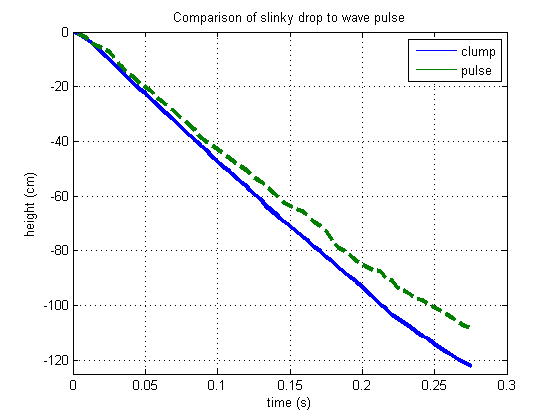
\includegraphics[scale=0.5]{figs/ClumpPulse}
\end{center}
\vspace{-4ex}
\caption{The position of a wave pulse on a suspended slinky compared to the position
of the top of an identical slinky when falling as a function of time.}
\label{fig:clumppulse}
\end{figure*}

The results of the measurements are shown in \fig{clumppulse}. These measurements
make clear that the falling top clump moves faster than a wave pulse on the same
slinky would. This becomes a very intuitive way of understanding the
slinky drop. First, we understand that information travels at finite speed and so
the news of the release of the slinky will take time to propagate down the slinky.
Second, we find that the collapse of the medium exceeds the speed at which
the wave pulse is capable of carrying the information. This explains why the
bottom will still be stationary when the top arrives.

\section{Discussion of Two Models}
\label{sec:discussion}

%% Old line from intro
% Despite the conceptual simplicity of the discrete model, the explanation
% required a large number of logical steps and a difficult calculation to arrive at
% the final conclusion. 


\NOTE{Comparing the physical realization of the model to the slinky 
helps emphasize the distinction between the model and the actual phenomenon of interest.}

\NOTE{Possible sentence: Just as we gained insight from looking at different models, we also benefited from
having students with diverse backgrounds who were able to provide different
perspectives on the problem.}

\NOTE{This sentence was moved from Section 3: This model for the slinky contrasted nicely with the previous model. The students were now thinking about
the slinky as a continuous object rather than a set of connected parts.}

The fact that the slinky drop lends itself so naturally to two very different models
makes it an excellent backdrop for teaching model building. Having explored both
models, students are able to compare and contrast what kinds of insight are
offered by each one. Which model seems to apply more directly to the overarching
question of the ``levitation?'' Which model uses more basic concepts? Which model
better allows one to see the intermediate evolution of the slinky as it falls?
The models use different fundamental concepts and rules and approach
the problem in very different ways, yet obtain consistent results.

Students often approach physics assuming that there is a single ``correct'' way
of looking at a problem. We sought to combat any expectation that we would
provide the ``right'' well-defined model and leave the students to solve it within
comfortable boundaries.
The students constructed a model on their own from basic underlying
principles, figuring out different perspectives that could be taken, selecting which effects
to take into account, and determining which approximations to make.
\TODO{Lots of references are warranted in this paragraph. (Ryan)}

\NOTE{Add paragraph about the process of model building and what is learned there. (Jesse)}

In both models, students can develop, test, and refine their models in an iterative process.
This presents the idea that a physical model is not static, but can undergo revision and development.
The development of the models follows closely to the definition of a model presented by Hestenes\cite{hestenes1987}. First students develop the object and descriptors that are the building blocks of their model.
This involves making decisions about what properties of the physical object need to be represented in the model.
Then students develop the equations of the model that determines how the model will behave.
Finally, the students must interpret the predictions of their model and compare it to the observations of the phenomenon.

We then took advantage of the slinky to force the students to attack the problem
from a different angle.\TODO{Reword this sentence} Constructing a different model showed the students
how the set of decisions they made the first time around was not necessarily
\emph{the} unique way of approaching the problem. Multiple acceptable and potentially
useful approaches were possible for describing the same phenomenon.

Each model makes different parts of the underlying physics
more transparent. The details of the interactions between the successive coils
of the slinky is manifest in the discrete model while the fundamental
limitation in the speed of information travel is less obscured in the model
using waves. Advantages of the discrete model included the students' ready
familiarity with the basic concepts of mechanics required and the straightforward
nature of the strategy of breaking the system into component parts. There were
fewer conceptual hurdles to overcome in this approach, and the mediating
reactions in the middle of the slinky were easy to see. 

Ultimately however, we feel that the information-based model provided the
most direct explanation for the levitation of the bottom of the slinky, albeit
using more sophisticated concepts. It focused
on the most relevant concepts for the question and abstracted away
nonessential parts. The great insight provided by the
model demonstrates the idea that the most useful models
capture only the effects that we are most interested in explaining.

Being able to readily attack the slinky drop from multiple angles, combined with
the fact that the slinky was simple enough to be approachable by the students
in a hands-on fashion, made it an ideal centerpiece of a curriculum intended to
introduce students to model building and allowed us to highlight many of the
essential features of model building in the physical sciences.


\acknowledgments The authors would like to acknowledge the support of the Compass
Project community and the UC Berkeley instructional support staff along with
helpful discussions with D. R. Dounas-Frazer and J. Corbo.
This work was supported by the Departments of Physics, Astronomy, and Earth and
Planetary Sciences at UC Berkeley and private donations.

\NOTE{Fix person and tense}

\NOTE{We will tend to reference things generically instead of about our students and tend to use present tense instead of past where possible, but in places where it preferrable to do it the other way, it is fine.}

\NOTE{Fix grammar and proofread!}

\NOTE{Update paper with terminology: ``slinky drop,'' ``top clump,'' ``wave pulse,'' leave references to the bottom as ``bottom'' if possible}

\bibliography{slinky_bibliography}

\end{document}
